\documentclass[aps,prl,reprint,amsmath,amssymb]{revtex4-1}

\usepackage{epsfig,color,graphicx}
%\usepackage{algorithmic}
\usepackage{algorithm}
\usepackage{algpseudocode}

% Mathematical symbols
\newcommand*{\imi}{i} % imaginary i
\newcommand*{\E}{\mathrm{e}}
% DIRAC NOTATION
% bra-ket vectors
\newcommand{\ket}[1]{\ensuremath{\vert #1 \rangle}}
\newcommand{\bra}[1]{\ensuremath{\langle #1 \vert}}
\newcommand{\braket}[2]{\ensuremath{\langle #1 \vert #2 \rangle}} % bra-ket inner product
\newcommand{\ketbra}[2]{\ensuremath{\vert #1 \rangle \langle #2 \vert}} % ket-bra outer product
% operators
\newcommand{\op}[1]{\ensuremath{\hat{#1}}} % operator
\newcommand{\opsb}[2]{\ensuremath{\hat{#1}_{#2}}} % operator with subscript
\newcommand{\opsp}[2]{\ensuremath{\hat{#1}^{#2}}} % operator with superscript

% left-right arrow with text above it
\makeatletter
\newcommand\xleftrightarrow[2][]{%
  \ext@arrow 9999{\longleftrightarrowfill@}{#1}{#2}}
\newcommand\longleftrightarrowfill@{%
  \arrowfill@\leftarrow\relbar\rightarrow}
\makeatother

% inexact differential
\def\dbar{{\mathchar'26\mkern-12mu d}}

%partial derivative with some variables held constant
\newcommand{\pdc}[3]{\ensuremath{\left( \frac{\partial #1}{\partial #2} \right)_{#3}}}
\newcommand{\pddc}[3]{\ensuremath{\left( \frac{{\partial}^2 {#1}}{\partial {#2}^2} \right)_{#3}}}

%average
\newcommand{\av}[1]{\ensuremath{\left\langle{#1}\right\rangle}} % operator

%text color
\newcommand{\new}{\color{red}}
\newcommand{\blue}{\color{blue}}
\newcommand{\old}{\color{black}}

\begin{document}

\bibliographystyle{apsrev}


\title{
Direct unconstrained localization of nonorthogonal one-electron orbitals
}

\author{Ziling Luo}
\email{ziling.luo@mail.mcgill.ca}
\author{Rustam Z. Khaliullin}
\email{rustam.khaliullin@mcgill.ca}
\affiliation{Department of Chemistry, McGill University, 801 Sherbrooke St. West, Montreal, QC H3A 0B8, Canada}

\date{\today}

\begin{abstract}
Spatially localized one-electron orbitals are of tremendous importance in electronic structure theory of materials and molecular systems. 
They are used to interpret chemical bonding and speed up computations. 
\end{abstract}

\maketitle

\section{Introduction} 

One-electron orbitals, which are defined as molecular orbitals (MOs) in the molecular systems and Bloch orbitals in the solid state field, play a paramount important role in electronic structure theory. 
Delocalized canonical molecular orbitals (CMOs) are widely implemented in current electronic structure calculations due to they have well defined energies and associated orbital energies. 

Localized MOs (LMOs) and their condensed-phase equivalent maximal localized Wannier functions (MLWFs) provide an equivalent description of the electron distribution in one-electron theories (Hartraa-Fock, Density Functional Theory) and are widely used to describe the chemical bonding patterns since the classical chemical bonding theory describes the bonding properties as the localized distributed electrons.
The conventional electronic structure methods experience high-cost and slow running time problems when applied to large systems, because of the need of the cubic scaling operation to diagonalize the Hamiltonian matrix.
To overcome the limitation, researchers have focused on developing the LS methods.
LMOs have been proposed to be an extremely promising candidate to achieve LS calculations in many local electron correlation electronic structure methods.~\cite{wang1992simple, ordejon1993unconstrained, mauri1993orbital, mauri1994electronic, stechel1994n_scaling, goedecker1994efficient}

Early developments of the LMOs were constrained to be orthogonal (OLMOs)~\cite{weinstein1971localized} which can be obtained through unitary transformations from CMOs based on extremizing the localization functions, such as Boys-Foster~\cite{boys1960construction}, Edmiston-Ruedenberg~\cite{bytautas2002electron, bytautas2003split, edmiston1963localized}, Pipek-Mezey~\cite{pipek1989a_fast}, and Von Niessen methods~\cite{niessen1972density}.
Due to the orthogonality condition of the OLMOs, the "orthogonalization tails" outside the localization center can be observed in the generated OLMOs.
These "orthogonalization tails" reduce the localization and complicated the electronic structural information transformation from one system to another.

Since nonorthogonal LMOs (NLMOs)~\cite{anderson1968self, diner1968fully, magnasco1974localized, payne1977hartree, mehler1977self} are obtained by nonsingular transformation from CMOs without the orthogonality condition, more degrees of freedom are available during the generation of NLMOs, resulting in a more localized distribution of electrons in space.
The concept of NLMOs was firs introduced by Anderson~\cite{anderson1968self} and Diner et al~\cite{diner1968fully} in 1968, but more efforts were devoted to constructing OLMOs previously.
Several efforts have been made to develop the method to construct NLMOs recently~\cite{feng2004An_efficient, liu2000nonorthogonal, peng2013effective, hoyvik2017generalising}, and researchers have proposed that NLMOs are about $10-30 \%$ more compact than OLMOs~\cite{feng2004An_efficient, liu2000nonorthogonal}.

One way to construct NLMOs is to employ the variational optimization by restricting the variational space to a local space.
The NLMO is then expanded in the variational space, which helps to eliminate the long-range tails.
However, this approach may introduce error due to the basis set truncation and lead to result in the very approximation NLMOs because the choice of the local space may be different from the true localization region.

Other studies proposed another method to obtain NLMOs by linear transformations of CMOs with relaxation of the orthogonality constraint.~\cite{feng2004An_efficient, cui2010efficient} 
The limitation of this method is that the final MOs either are still fairly orthogonal and similar localization compared with OLMOs or lead to the linear dependence between the orbitals.~\cite{feng2004An_efficient} (we will refer to the linear dependence problem as the collapse problem.)
To overcome the collapse problem, Yang and co-workers~\cite{feng2004An_efficient, cui2010efficient}  developed a method to construct NLMOs by fixing the centers of NLMOs during the minimization of the spread functional. 
The positions of the centers are predefined from the corresponding OLMOs~\cite{feng2004An_efficient} or good understanding of bonding patterns in the systems (i.e.``chemical intuition'')~\cite{cui2010efficient}.
While this method solved the linear dependence problem, it still needs more computational efforts to construct OLMOs centroids and to know the bonding properties in advance by using "chemical intuition", which may limit the application of the method.

In this paper, we propose a fully black box method to construct the NLMOs without the need of predefined centroids.
With the new approach, NLMOs can be obtained by automatic minimization the unconstrained spread functional with the  penalty functional which prevents the orbital collapse.
We successfully developed this new black-box approach to obtain NLMOs and achieved more compact and nonorthogonal MOs compared with OLMOs.

\section{Theory and algorithms}

The localization procedure starts with a set of occupied (or ZZZ virtual?) one-electron states $\ket{i_0}$. 
These orbitals are not assumed to be canonical or even orthogonal. 
However, they are assumed to be normalized. 
Furthermore, they must be linear independent, that is, their overlap matrix $\sigma_{ji}^0 \equiv \braket{j_0}{i_0}$ must be invertible. 
The trial NLMOs are expressed as a linear combination of these initial states
%
\begin{equation}
\begin{split}
\ket{j} = \ket{i_0} {A^i}_j  
\end{split}
\end{equation}
%
The conventional tensor notation is used to work with the nonorthogonal orbitals~\cite{head1998tensor}: covariant quantities are denoted with subscripts, contravariant quantities with superscripts, and summation is implied over the same orbital indices.

The objective function minimized in this work contains two terms: a conventional localization functional $\Omega_L$ and a term that penalizes unphysical states with linearly dependent occupied orbitals $\Omega_P$:
%
\begin{equation} \label{eq:fun-pen}
\begin{split}
\Omega(\mathbf{A}) = \Omega_L(\mathbf{A}) + c_P \Omega_P(\mathbf{A}), \\
\Omega_P(\mathbf{A}) = - \log \det \left[ \sigma (\mathbf{A}) \right]
\end{split}
\end{equation}
%
where $c_P > 0$ is the penalty strength, $\sigma$ is the NLMO overlap matrix 
%
\begin{equation}
\begin{split}
\sigma_{kl} = \braket{k}{l} = {A^j}_k \sigma_{ji}^0{A^i}_l
%= (\mathbf{A}^\dagger \mathbf{T}^\dagger \mathbf{ S T A})_{kl},
\end{split}
\end{equation}
%

If the NLMOs are normalized the determinant of $\sigma$ varies from 1 for orthogonal NLMOs to 0 for linearly dependent NLMOs. The penalty function---the key ingredient of the proposed method---varies from 0 to $+\infty$ for these two extreme cases, making linearly dependent state inaccessible in the localization procedure with finite penalty strength $c_P$. 
% RZZK: Why sigma instead of A? quadratic penalty in terms of A (more complicated in terms of a). Why log?
A normalization constraint can be imposed on NLMOs if their coefficients are expressed in terms of independent variational parameters denoted with lowercase $\mathbf{a}$
%
\begin{equation}
\begin{split}
{A^i}_j = {a^i}_{j} ({a^k}_{j} \sigma^0_{kl}{a^l}_{j})^{-\frac{1}{2}}
\end{split}
\end{equation}
%
The inclusion of the penalty term converts the localization procedure into an unconstrained and straightforward optimization problem. Additionally, adjusting the strength of the penalty $c_P$ enables one to achieve the right balance between the nonorthogonality and locality of the orbitals. 
%RZK: We will demonstrate below that this flexibility is useful because a high degree of linear dependence  
A procedure that finds the penalty strength for the desired compromise between the nonorthogonality and locality is discussed below. 

In this work, we adopted the following localization functional 
%
\begin{equation} \label{eq:fun-loc}
\begin{split}
\Omega_L(\mathbf{A}) &= - \sum_K \sum_i \omega_K \log \vert z_{i}^{K} \vert^2, \\
z_{i}^{K} &= {A^m}_i B^{K}_{mn} {A^n}_i, \\
B^{K}_{mn} &= \bra{m_0} \E^{\imi \mathbf{G}_K \cdot \mathbf{\op{r}}} \ket{n_0}
\end{split}
\end{equation}
%
%RZZK - K is an upper index that is not contravariant, there is also covariant K
%RZZK - minus sign ensures minimization vs maximazation
%RZZK - use other functions?
%RZZK - Explain how Boys functions are obtained.
where $\omega_K$ , $\mathbf{G}_K$, $\mathbf{\op{r}}$ - RZK. Summation over $K$ is written out explicitly because $K$ is not an orbital index. This functional can be used for both periodic (ZZZ at $\Gamma$-point only?) and gas-phase systems~\cite{berghold2000general}. In the latter case, it is equivalent to the Boys localization functional~\cite{RZK}.
% berghold2000general --- PHYSICAL REVIEW B, 61,

There exists a multitude of algorithms to carry out the unconstrained minimization of functional $\Omega$ with fixed $c_P$. In this work, we used a simple conjugate gradient algorithm summarized in Figure~\ref{fig:cg}. The gradient ${G_i}^j \equiv \frac{\partial \Omega}{\partial {a^i}_j}$  required in the algorithm is a sum of the localization ${L_i}^j \equiv \frac{\partial \Omega_L}{\partial {a^i}_j}$ and penalty ${P_i}^j \equiv \frac{\partial \Omega_P}{\partial {a^i}_j}$ components
%
\begin{equation} \label{eq:grad}
\begin{split}
G{_k}^{l} = L{_k}^{l} + c_P P{_k}^{l}.
\end{split}
\end{equation}
%
These components can be readily expressed in terms of the derivatives with respect to the transformation coefficients $\tilde{X}{_k}^l \equiv \frac{\partial \Omega_X}{\partial {A^k}_l}$, where $X$ is either $L$ or $P$:
%
\begin{equation} \label{eq:grad-convert}
\begin{split}
{X_i}^j & = \tilde{X}{_k}^l \frac{\partial {A^k}_l}{\partial {a^i}_j} = \tilde{X}{_i}^j \sigma_{jj}^{-\frac{1}{2}} - \sigma_{in}^0 {A^n}_j  \sigma_{jj}^{-\frac{1}{2}} {A^m}_j \tilde{X}{_m}^j
\end{split}
\end{equation}
%
\begin{equation} \label{eq:grad-loc}
\begin{split}
\tilde{L}{_k}^l & = - \sum_K \frac{4 \omega_K}{\vert z_{l}^{K} \vert^2} \times \\ 
&\times \left[  \operatorname{Re}(B^{K}_{kn}) {A^{n}}_{l} \operatorname{Re}(z_{l}^{K}) + \operatorname{Im}(B^{K}_{kn}) {A^{n}}_{l} \operatorname{Im}(z_{l}^{K}) \right]
\end{split}
\end{equation}
%
\begin{equation} \label{eq:grad-pen}
\begin{split}
\tilde{P}{_k}^l & = -2 \sigma_{km}^0 {A^m}_n \sigma^{nl} 
\end{split}
\end{equation}
%

\textbf{Adjusting penalty strength.} In the case of extremely large $c_P$, $\Omega_L$ is negligible compared to the penalty term and the minimization of $\Omega$ is equivalent to a trivial orbital orthogonalization. In the opposite case of extremely small $c_P$, the minimization of $\Omega$ leads to a linear dependence between NLMOs and the failure of the algorithm in Figure~\ref{fig:cg}. % to invert the NLMO overlap in Eq.~(\ref{eq:grad-pen}). 
The strategy of finding the optimal penalty strength adopted in this work is to use moderately large initial $c_P$ value and perform the minimization of $\Omega$ gradually decreasing $c_P$ until the value of the determinant of the NLMO overlap drops below a desired threshold value $\epsilon_{\text{Det}} \in (0,1)$. The initial value of $c_P$ is chosen so that the 
%
\begin{equation}
\begin{split}
c_{P} \gets - \Omega^0_{L}(\Omega^0_P + \log \epsilon_{\text{Det}})^{-1}  
\end{split}
\end{equation}
%
The logic behind this equation: but the functional before optimization must be larger than after 
%
\begin{equation}
\begin{split}
\Omega^0_{L} + c_P \Omega^0_P > \Omega^{\text{expected}}_L - c_P \log \epsilon_{\text{Det}} 
\end{split}
\end{equation}
%
which results in
%
\begin{equation}
\begin{split}
c_P > (\Omega^{\text{expected}}_L - \Omega^0_{L}) (\Omega^0_P + \log \epsilon_{\text{Det}})^{-1}
\end{split}
\end{equation}
%
At the same time, the initial $c_P$ value must be as small as possible.

{\color{red} It might seem like a good idea to choose initial $c_P$ value that minimizes the Frobenius norm of the total gradient. The motivation is that the gradient of the localization component can be balanced as much as possible by the penalty gradient. In this case, the initial $c_P$ is given by the equation below (somewhat problematic index summation). The main reason not to use this initial value is that for $P_k^l$ is zero for all orthonormal states, giving infinitely large coefficient.
%
\begin{equation}
\begin{split}
c_P = - \frac{ \sum_{nm} {L_m}^n {P_m}^n}{ \sum_{kl} {P_k}^l {P_k}^l}  
\end{split}
\end{equation}
%
}


\begin{figure}
\begin{algorithm}[H]
  \caption{Conjugate gradient minimization of $\Omega$}
  \label{alg:cg}
   \begin{algorithmic}[1]
   	%\Procedure{Minimize$\Omega$}{$c_P, \tau, \mathbf{T}_0$}
	\State Input $\epsilon_{\text{CG}}$ \Comment{Localization convergence threshold}
	%\State Input $N_{\text{CG}}$, $N_{\text{Outer}}$ \Comment{Max CG, outer iterations}
	\State Input $\epsilon_\text{Det}$ \Comment{Minimum allowed NLMO determinant}
   	\State Input $\mathbf{T}_0$ \Comment{Coefficients of the initial states $\ket{i_0}$}
   	\State Input $\mathbf{S}$ \Comment{Basis set overlap}
   	\State Input $\mathbf{L}^K$ \Comment{Basis set representation of the localization operator} 
   	%RZZK: Localization matrix L is not defined. Loop over K?
   	\State $\mathbf{\sigma}_0 \gets \mathbf{T}_0^{\dagger} \mathbf{ST}_0$ \Comment{Initial orbital overlap} 
   	\State $\mathbf{B}^{K} \gets \mathbf{T}_0^{\dagger} \mathbf{L}^K \mathbf{T}_0$ \Comment{Initial localization matrix} 
	\State $\mathbf{a} \gets \mathbf{I}$ \Comment{Guess variational DOFs}
	%\State Converged $\gets$ False
	\State StopOuter $\gets$ False \Comment{Flag to exit the outer loop}
	\State $i_{\text{Outer}} \gets 0$ \Comment{Iteration counter}
	\Repeat \Comment{Loop to change the penalty strength}
		\State $i_{\text{Outer}} \gets i_{\text{Outer}} + 1$ 
		\If{$i_{\text{Outer}}>1$} \Comment{$c_P$ is initialized below}
			\State $c_{P} \gets c_P / 2$ 
		\EndIf
		\State StopCG $\gets$ False \Comment{Flag to exit the CG loop}
		\State $i_{\text{CG}} \gets 0$ \Comment{Iteration counter}
%		\State $\beta \gets 0$ \Comment{Reset conjugation}
		\Repeat \Comment{Fixed-penalty localization loop}
			\State $i_{\text{CG}} \gets i_{\text{CG}} + 1$ 
			\State $\mathbf{A} \gets \mathbf{a} \left[ \text{diagonal}(\mathbf{a}^{\dagger} \mathbf{\sigma}_0 \mathbf{a}) \right]^{-\frac{1}{2}}$ \Comment{Update NLMOs}
			\State $\mathbf{\sigma} \gets \mathbf{A}^{\dagger}\mathbf{\sigma}_0 \mathbf{A}$ \Comment{Update overlap}
			\State $\text{Det} \gets \text{determinant} (\mathbf{\sigma})$ \Comment{Determinant}
			\State $\Omega_{P} \gets - \log [\text{Det}] $ \Comment{Orthogonalization functional}
			\State $\mathbf{P} \gets \text{Eq~(\ref{eq:grad-pen}) and~(\ref{eq:grad-convert})}$ \Comment{Orthogonalization gradient}
			\State $\Omega_{L} \gets \text{Eq~(\ref{eq:fun-loc})}$ \Comment{Localization functional}
			\State $\mathbf{L} \gets \text{Eq~(\ref{eq:grad-loc}) and~(\ref{eq:grad-convert})}$ \Comment{Localization gradient}
			\If{$i_{\text{Outer}}=1$ \textbf{and} $i_{\text{CG}}=1$} 
				%\State $c_{P} \gets \text{Tr}(\mathbf{L}^{\dagger} \mathbf{P})/\text{Tr}(\mathbf{P}^{\dagger}\mathbf{P})$
				\State $c_{P} \gets - \Omega_{L}(\Omega_P + \log \epsilon_{\text{Det}})^{-1}$ \Comment{Initial strength}
			\EndIf
			\State $\Omega \gets \Omega_{L} + c_P \Omega_{P} $ 
			\If{$i_{\text{CG}}>1$}
				\State $\mathbf{\Gamma} \gets \mathbf{G}$ \Comment{Save old gradient}
			\EndIf 
			\State $\mathbf{G} \gets \mathbf{L} + c_P \mathbf{P} $ 
			%\State $\text{Error}_\text{CG} \gets \vert\vert \mathbf{G} \vert \vert_{\text{max}}$
			\If{$\vert\vert \mathbf{G} \vert \vert_{\text{max}} < \epsilon_{\text{CG}}$}
				\State StopCG $\gets$ True
			\EndIf
%			\If{$i_{\text{CG}}=1$ \textbf{And} $i_{\text{Outer}}=1$}
%				\State StopCG $\gets$ False \Comment{Do first iteration}
%			\EndIf
			\If{\textbf{not} StopCG}
%				\If{$i_{\text{CG}} = 1$}
%					\State $\mathbf{P}^{R_c} \gets \text{Eq.\ref{eq:prec}}(\mathbf{F},\mathbf{M}^{R_c},\mathbf{K}^{R_c}) $\Comment{Precon.}
%				\Else
%					\State $\mathbf{O}_{R_c} \gets \mathbf{D}_{R_c}$ \Comment{Save old direction}
%				\EndIf
				\If{$i_{\text{CG}} > 1$}
					\State $\mathbf{O} \gets \mathbf{D}$ \Comment{Save old direction}
				\EndIf
%				\State $\mathbf{D}_{R_c} \gets - [(\mathbf{P}^{R_c})^{-1} \mathbf{G}^{R_c}]_{R_c}$ \Comment{Precon. grad.}
				\State $\mathbf{D} \gets - \mathbf{G}$ \Comment{Initial direction}
				\If{$i_{\text{CG}}>1$}
					\State $\beta \gets \text{Tr}(\mathbf{G}^{\dagger} \mathbf{D})/\text{Tr}(\mathbf{\Gamma}^{\dagger}\mathbf{O})$
					\State $\mathbf{D} \gets \mathbf{D} + \beta \mathbf{O}$ \Comment{Search direction}
				\EndIf 
				\State $\alpha \gets \text{argmin}_{\alpha} \Omega(\mathbf{a} + \alpha \mathbf{D})$ \Comment{Line search}
				\State $\mathbf{a}\gets \mathbf{a} + \alpha \mathbf{D}$ \Comment{Update variational DOFs}
			\EndIf
		\Until{StopCG} 
		%\If{$\text{Det} < \text{Det}_{\text{Target}}$ \textbf{or} $i_{\text{Outer}} > N_{\text{Outer}}$}
		\If{$\text{Det} < \epsilon_{\text{Det}}$}
			\State StopOuter $\gets$ True
		\EndIf
	\Until{StopOuter}
	\State $\mathbf{return}$ $\mathbf{T} \gets \mathbf{T}_0 \mathbf{A} $ \Comment{Return NLMOs coefficients}
	%\EndProcedure
   \end{algorithmic}
\end{algorithm}
\caption{\label{fig:cg} Algorithm for the optimization of NLMOs.}
\end{figure}


\section{Results and discussion}
\begin{table}[ht]
\caption{The Localization functional, final determinant and relative percentage of NLMOs compared with OLMOs}
\centering
\begin{tabular}{c c c c c}
\hline\hline
Molecules & CMO &  OLMO$(\%)$ & NLMO$(\%)$ & Final Determinant \\
\hline
H$_2$O& 363 & 288 (20.5) & 230 (20.3) & 0.263 \\ 
C$_3$H$_6$ & 2259 & 883 (60.9) & 747 (15.4) & 1.131E-06 \\ 
B$_2$H$_6$ & 1727 & 676 (60.9) & 630 (6.7) & 0.718 \\ 
C$_6$H$_6$  & 5676 & 1727 (69.6) & 1157 (33.0) & 5.721E-06 \\ 
C$_7$H$_{16}$ & 20016 & 2220 (88.9) & 1953 (12.0) & 0.122 \\ 
C$_2$B$_{10}$H$_{12}$ & 11830 & 3432 (71.0) & 2813 (18.1) & 0.004 \\ 
C$_{20}$H$_{42}$ & 245277 & 6160 (97.5) & 5405 (12.2) & 0.003 \\ 
C$_{72}$H$_{24}$ & 351937 & 22791 (93.5) & 15773 (30.8) & 1.925E-07 \\ 
Graphene & 34998 & 8025 (77.1) & 5281 (34.2) & 2.176E-07\\
Average & & 71.1 & 20.3 & \\
\hline
\end{tabular}
\label{table:nonlin}
\end{table}

\begin{figure}[htbp]
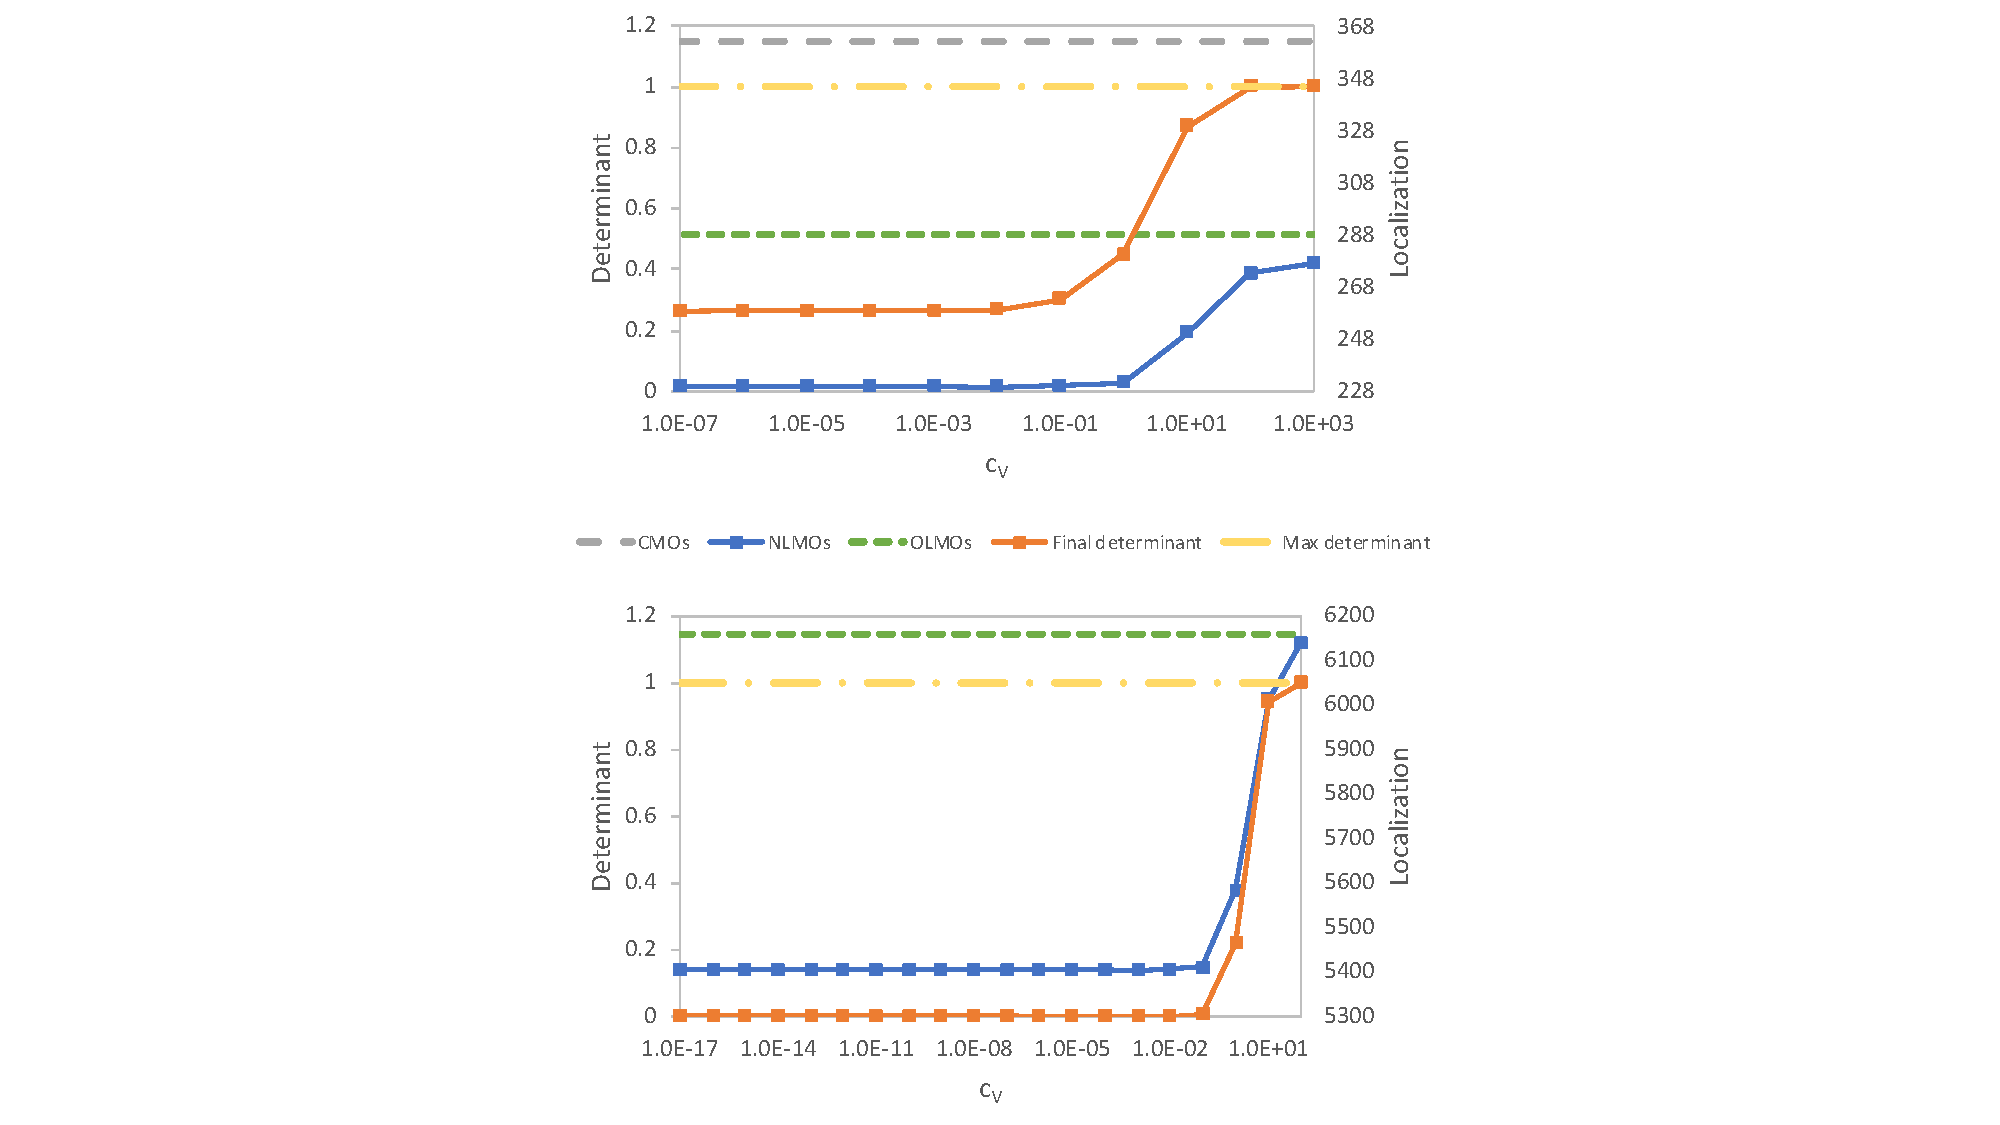
\includegraphics[scale=0.65]{figure_1.pdf} 
  \caption{The localization function vs Volume penalty coefficient of water molecule}
\end{figure}

To test our newly generated method, we performed the simulation on several systems from simple water molecule to large polymers (H$_2$O, C$_3$H$_6$, B$_2$H$_6$, C$_6$H$_6$, C$_7$H$_{16}$, C$_2$B$_{10}$H$_{12}$, C$_{20}$H$_{42}$ and C$_{72}$H$_{24}$).

We employed the DFT method to determine the NLMOs and calculate the related quantities (localization functional, determinant of CMOs, OLMOs and NLMOs).

The optimization is stable and relative efficient in all out tests.

The results are showed in the Table 1. 

To illustrate the extent of the localization,  the Boys localization functional is calculated to compare between CMOs, OLOMOs and NLMOs.

The determinant is reported to describe the orthogonality, which is related to the linear dependence issue.

The results of localization functional of the CMOs, OLMOs and NLMOs are tabulated in columns of 2-4 of table 1, respectively.

The relative decreases of the localization functions of the NLMOs to OLMOs are also reported in the table, which are from $6.7\%$ to $34.2\%$ and $20.3\%$ on average.

The final determinant value has showed that all obtained NLMOs are linear independent and do not collapse onto each other.

By visualizing the generated NLMOs and OLMOS, we compare the spatial difference between them with the classical chemical bonding principles.

We present several representative examples and show the shape of NLMOs and OLMOs.


\begin{figure*}[hbpt]
\centering
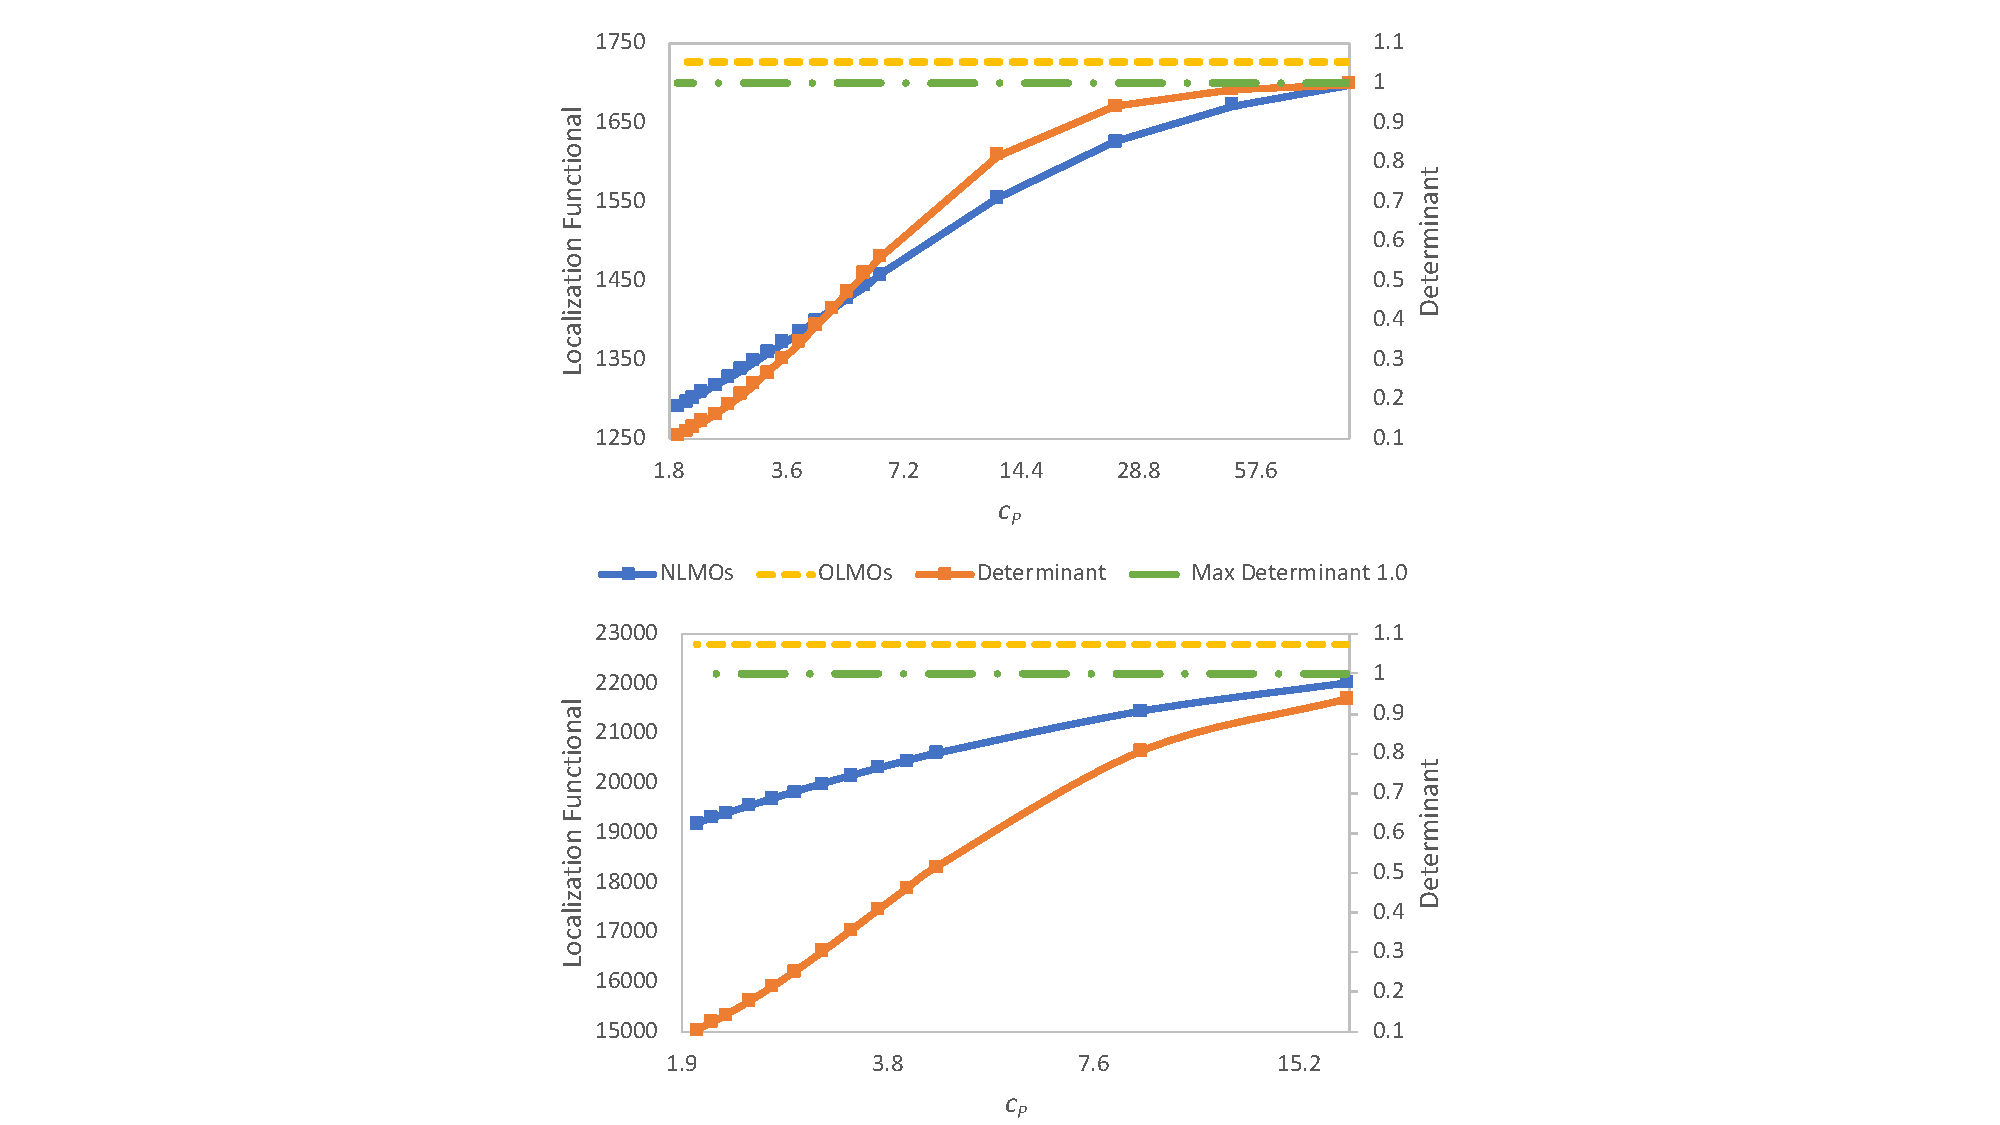
\includegraphics[width=\textwidth]{figure_2.pdf}
\caption{The localization function vs Volume penalty coefficient of tested molecules}
\end{figure*}

% This file is not in the repository
%\begin{figure}[htbp]
%\includegraphics[scale=0.2]{nlmo_C2B10H12_1.pdf} 
%  \caption{The localization function vs Volume penalty coefficient of tested molecules}
%\end{figure}

After comparing the 

Present localization paths for two systems: simple and challenging. Use $c_P$ values determined by our automatic procedure. Remember that the whole point of creating this method was to make the localization black-box.

Can we localize virtual orbitals?

Present a table that compares orthogonal and nonorthogonal results, final determinants.

Show localization orbitals for a big molecule, molecule with non-intuitive electronic structure, and a periodic material.

Discuss existing issues: convergence rate, sigma-pi mixing, orthogonalization tails, sparsity of the final coefficients. Mention possible future work to resolve them.

TODO: Visualize an xyz file with localization centers to make sure NLMOs are physical. Compute the $c_P$ coefficient correctly the equation to minimize the L2 norm of the gradient.

check the coordinated of the localized orbital centres???

\section{Conclusions}


\section{Computational details}


\section{Acknowledgments} 

The research was funded by the Natural Sciences and Engineering Research Council of Canada (NSERC) through Discovery
Grants (RGPIN-2016-0505). The authors are grateful to Compute Canada and, in particular, the McGill HPC Centre for computer time.

\bibliographystyle{apsrev4-1}
\bibliography{NLMO}

\end{document}
